\documentclass[11pt,oneside]{article}

\usepackage[T1]{fontenc}
\usepackage[utf8]{inputenc}
\usepackage{mathtools,amsthm}
\usepackage{newtxtext,newtxmath}
\usepackage{microtype}
\usepackage[margin=1.08in]{geometry}
\usepackage{booktabs,tabularx,array,longtable}
\usepackage{enumitem}
\usepackage{xcolor}
\usepackage[most]{tcolorbox}
\usepackage{tikz}
\usetikzlibrary{arrows.meta,positioning,calc,fit}
\usepackage{fancyhdr}
\usepackage{titlesec}
\usepackage{hyperref}
\usepackage{bookmark}
\usepackage[nameinlink,noabbrev]{cleveref}

\definecolor{navy}{HTML}{17365D}
\definecolor{teal}{HTML}{0D6B66}
\definecolor{burgundy}{HTML}{7C2431}
\definecolor{gold}{HTML}{B07A11}
\definecolor{softblue}{HTML}{EEF4FA}
\definecolor{softgreen}{HTML}{EDF8F4}
\definecolor{softred}{HTML}{FAF0F1}
\definecolor{softgold}{HTML}{FBF6E9}
\definecolor{darkgray}{HTML}{333333}

\hypersetup{
  colorlinks=true,
  linkcolor=navy,
  citecolor=teal,
  urlcolor=burgundy,
  pdftitle={A Universal-Cover and Entire-Interpolation Attack on the Alaoglu--Erdos Conjecture},
  pdfauthor={OpenAI, mathematical research report},
  pdfsubject={Alaoglu--Erdos conjecture, four exponentials, q-difference equations, integer-valued entire functions},
  pdfkeywords={Alaoglu--Erdos, four exponentials, canonical products, entire interpolation, monodromy}
}

\pagestyle{fancy}
\fancyhf{}
\fancyhead[L]{\small\sffamily\color{navy}Alaoglu--Erd\H{o}s: universal-cover attack}
\fancyhead[R]{\small\sffamily\color{navy}\nouppercase{\leftmark}}
\fancyfoot[C]{\small\sffamily\thepage}
\setlength{\headheight}{14pt}

\titleformat{\section}
  {\Large\bfseries\sffamily\color{navy}}{\thesection}{0.65em}{}
\titleformat{\subsection}
  {\large\bfseries\sffamily\color{teal}}{\thesubsection}{0.65em}{}
\titleformat{\subsubsection}
  {\normalsize\bfseries\sffamily\color{burgundy}}{\thesubsubsection}{0.65em}{}

\setlist[itemize]{leftmargin=1.6em,itemsep=0.25em,topsep=0.35em}
\setlist[enumerate]{leftmargin=1.8em,itemsep=0.35em,topsep=0.4em}
\setlength{\parindent}{0pt}
\setlength{\parskip}{0.55em}

\newtheorem{theorem}{Theorem}[section]
\newtheorem{proposition}[theorem]{Proposition}
\newtheorem{lemma}[theorem]{Lemma}
\newtheorem{corollary}[theorem]{Corollary}
\newtheorem{criterion}[theorem]{Criterion}
\theoremstyle{definition}
\newtheorem{definition}[theorem]{Definition}
\newtheorem{problem}[theorem]{Problem}
\newtheorem{experiment}[theorem]{Experiment}
\theoremstyle{remark}
\newtheorem{remark}[theorem]{Remark}
\newtheorem{warning}[theorem]{Warning}

\newtcolorbox{verdictbox}{
  enhanced,breakable,
  colback=softred,colframe=burgundy,
  boxrule=0.8pt,arc=2mm,
  title={\bfseries\sffamily Research verdict},
  fonttitle=\color{burgundy},
  left=2mm,right=2mm,top=1.5mm,bottom=1.5mm
}
\newtcolorbox{resultbox}{
  enhanced,breakable,
  colback=softgreen,colframe=teal,
  boxrule=0.8pt,arc=2mm,
  title={\bfseries\sffamily Result established in this report},
  fonttitle=\color{teal},
  left=2mm,right=2mm,top=1.5mm,bottom=1.5mm
}
\newtcolorbox{gapbox}{
  enhanced,breakable,
  colback=softgold,colframe=gold,
  boxrule=0.8pt,arc=2mm,
  title={\bfseries\sffamily Exact remaining gap},
  fonttitle=\color{gold!70!black},
  left=2mm,right=2mm,top=1.5mm,bottom=1.5mm
}
\newtcolorbox{auditbox}{
  enhanced,breakable,
  colback=softblue,colframe=navy,
  boxrule=0.7pt,arc=2mm,
  title={\bfseries\sffamily Gap audit},
  fonttitle=\color{navy},
  left=2mm,right=2mm,top=1.5mm,bottom=1.5mm
}

\newcommand{\N}{\mathbb N}
\newcommand{\Nzero}{\mathbb N_0}
\newcommand{\Z}{\mathbb Z}
\newcommand{\Q}{\mathbb Q}
\newcommand{\R}{\mathbb R}
\newcommand{\C}{\mathbb C}
\newcommand{\Qbar}{\overline{\mathbb Q}}
\newcommand{\cO}{\mathcal O}
\newcommand{\cM}{\mathcal M}
\newcommand{\Log}{\operatorname{Log}}
\newcommand{\ord}{\operatorname{ord}}
\newcommand{\Span}{\operatorname{span}}
\newcommand{\e}{\mathrm e}
\newcommand{\dd}{\,\mathrm d}
\newcommand{\AEconj}{Alaoglu--Erd\H{o}s}
\newcommand{\FEC}{Four Exponentials Conjecture}
\newcommand{\fall}[2]{(#1)_{#2}}

\begin{document}

\hypersetup{pageanchor=false}
\begin{titlepage}
\centering
\vspace*{1.15cm}
{\sffamily\bfseries\color{navy}\fontsize{25}{30}\selectfont
A Universal-Cover and Entire-Interpolation Attack\par
on the Alaoglu--Erd\H{o}s Conjecture\par}
\vspace{0.55cm}
{\sffamily\Large\color{teal}
Local dilation rigidity, arithmetic monodromy,\par
and a sharp logarithmic-growth threshold}
\vspace{1.2cm}

\begin{tcolorbox}[width=0.91\textwidth,colback=softblue,colframe=navy,arc=2mm,boxrule=0.9pt]
\centering
\large
\[
2^x,3^x\in\Z \quad\Longrightarrow\quad x\in\Z\,?
\]
\end{tcolorbox}

\vspace{1.0cm}
{\large\sffamily Detailed gap-audited research report}\par
\vspace{0.25cm}
{\normalsize\sffamily Literature checked through 21 August 2026}\par
\vfill

\begin{minipage}{0.88\textwidth}
\small
\textbf{Scope.} This document is a new, self-contained continuation rather than a rewrite of the supplied unified report.  It deliberately does not repeat that report's large formalized corpus, conditional solution monoids, determinant catalogues, finite scans, valuation lattices, mixed-Mahler series, or matrix-coefficient reformulations.  The focus here is the actual power germ on the universal cover of \(\C^*\), its descent at the puncture, and an entire-interpolation formulation with an exact sharp growth constant.
\end{minipage}

\vspace{0.75cm}
{\small\sffamily Prepared as an independent mathematical research note}\par
\end{titlepage}
\hypersetup{pageanchor=true}
\pagenumbering{roman}

\begin{abstract}
Let \(x\in\R\) and suppose that \(M=2^x\) and \(A=3^x\) are integers.  The requested implication \(x\in\Z\) is a classical open problem and a special case of the Four Exponentials Conjecture.  This report does not assert a nonexistent unconditional proof.  Instead, it develops a distinct local-analytic attack and proves several exact results that sharply isolate what such a proof must accomplish.

On the universal cover \(w\mapsto \e^w\) of \(\C^*\), the power germ is \(F_x(w)=\e^{xw}\) and satisfies two translation equations with algebraic-integer multipliers,
\[
F(w+\log2)=M F(w),\qquad F(w+\log3)=A F(w).
\]
We prove that these two equations rigidly determine every nonzero entire solution upstairs: it must be \(C\e^{xw}\).  We then completely classify single-valued meromorphic solutions downstairs on \(\C^*\): they exist only when \(x\in\Z\), and are monomials.  Thus all remaining arithmetic difficulty is exactly a descent/monodromy problem, not a functional-equation problem.

A second contribution is a sharp P\'olya-type entire-interpolation criterion.  Put
\(\mathcal S=\{2^a3^b:a,b\ge0\}\).  Its canonical product
\[
E(z)=\prod_{a,b\ge0}\left(1-\frac{z}{2^a3^b}\right)
\]
has exact cubic logarithmic growth
\[
\log M_E(R)=\frac{(\log R)^3}{6\log2\log3}+O((\log R)^2).
\]
Any nonzero entire function vanishing on \(\mathcal S\) has at least the same leading growth.  Consequently, if the data
\(H(2^a3^b)=M^aA^b\) admit an entire interpolant with cubic logarithmic type strictly below
\(1/(6\log2\log3)\), then the dilation defects vanish identically, \(H\) is a monomial, and \(x\) is a nonnegative integer.  The constant is optimal for integrality alone, because \(1+E\) is a transcendental entire function taking the integer value \(1\) at every point of \(\mathcal S\) and attaining the critical type.

At the exact critical boundary, we factor the two dilation defects uniquely as \(D_2=EU\) and \(D_3=EV\).  The quotients satisfy a commuting cocycle involving explicit one-dimensional edge products of quadratic logarithmic growth.  Their unequal edge constants yield a second closure theorem: if \(U\) and \(V\) are polynomials, then both defects vanish and the interpolant is a monomial, even though the interpolant itself may have critical cubic type.

We also prove an arithmetic regularity ladder (meromorphic, Puiseux, algebraic, and \(\Qbar\)-D-finite germs), an elementary \(\Qbar\)-D-finiteness criterion for \(z^x\), an explicit nonlinear differential-equation false lead, and a strengthened monodromy statement from the Six Exponentials Theorem: under a counterexample, the branch multiplier \(\e^{2\pi i x}\) is transcendental, its powers are \(\Qbar\)-linearly independent, and the nonprincipal branch values over every divisible \(3\)-smooth base are all transcendental.  The final section gives a precise claim ledger and identifies four explicit bridges: subcritical interpolation, finite-dimensional divided defects at critical type, arithmetic holonomicity, or algebraic monodromy/descent.
\end{abstract}

\tableofcontents
\clearpage
\pagenumbering{arabic}

\section{Mandate, status, and claim discipline}

\subsection{The problem}

The \AEconj{} conjecture asks whether
\begin{equation}
  x\in\R,\qquad 2^x\in\Z,\qquad 3^x\in\Z
  \quad\Longrightarrow\quad x\in\Z.
  \label{eq:AE}
\end{equation}
Write throughout
\begin{equation}
  M:=2^x,\qquad A:=3^x.
  \label{eq:MA}
\end{equation}
The letters \(M,A\) are fixed positive integers whenever \eqref{eq:AE}'s hypotheses hold.

\begin{verdictbox}
As of the literature check dated 21 August 2026, the implication \eqref{eq:AE} remains open.  Waldschmidt's survey states this exact question and explains that a positive answer follows from the Four Exponentials problem \cite{Waldschmidt2023}.  The 2026 paper of Dasgupta and Kakde introduces the Matrix Coefficient Conjecture, whose \(2\times2\) case is equivalent to Four Exponentials, and explicitly leaves a needed implication open \cite{DasguptaKakde2026}.  Massold's 2025 work proves a weaker transcendence-degree estimate and reduces a stronger estimate to another major conjecture rather than settling the \(2\times2\) case \cite{Massold2025}.

Accordingly, an unconditional proof is not claimed below.  Every theorem marked as proved is proved in full; every use of a classical transcendence theorem is named; and the remaining bridge is stated explicitly rather than hidden in an auxiliary lemma.
\end{verdictbox}

\subsection{What is new here relative to the supplied report}

The supplied report is exceptionally broad.  It already treats the Four Exponentials reduction, conditional solution monoids, determinant and interpolation methods, valuation and \(p\)-adic obstructions, mixed Mahler series, automaticity, point counting, and extensive machine-checked partial results.  Repeating those chapters would add bulk rather than knowledge.

This continuation instead develops six pieces not developed there as a unified route:
\begin{enumerate}[label=\textbf{N\arabic*.}]
\item the exact classification of the two-dilation system on the \emph{universal cover} and on \(\C^*\);
\item a hierarchy of descent categories for the actual germ \(z^x\), including a direct \(\Qbar\)-D-finiteness theorem;
\item an explicit canonical product on the reciprocal \(3\)-smooth sampling set, showing why the identity theorem and weak growth restrictions fail;
\item the exact cubic logarithmic growth constant \(1/(6\log2\log3)\);
\item a sharp subcritical entire-interpolation theorem that would force \(x\in\Z\);
\item an exact critical-boundary defect cocycle and a polynomial-quotient closure theorem.
\end{enumerate}

\subsection{Proof-status vocabulary}

We distinguish the following.
\begin{itemize}
\item \textbf{Unconditional theorem}: proved here from stated hypotheses.
\item \textbf{Classical input}: a named theorem such as Gelfond--Schneider or Six Exponentials.
\item \textbf{Equivalent target}: a reformulation whose proof would settle \eqref{eq:AE}, but which is not itself established.
\item \textbf{No-go audit}: a rigorous explanation that a tempting inference is invalid or too weak.
\end{itemize}
This discipline matters at the Four Exponentials boundary, where a missing regularity hypothesis can turn a correct theorem into a false proof in a single line.

\section{Minimal arithmetic reductions}

Only the reductions needed for the new analytic route are recorded.

\begin{lemma}[Sign and rational exponents]
\label{lem:basic}
Assume \eqref{eq:AE}'s hypotheses.
\begin{enumerate}[label=(\roman*)]
\item \(x\ge0\).
\item If \(x\in\Q\), then \(x\in\Nzero\).
\item Therefore a nonintegral solution is irrational.
\end{enumerate}
\end{lemma}

\begin{proof}
If \(x<0\), then \(0<2^x<1\), so \(2^x\) cannot be an integer.  Thus \(x\ge0\).

Write \(x=p/q\) in lowest terms with \(q>0\).  If \(2^{p/q}=M\in\Z\), then
\(M^q=2^p\).  Taking the \(2\)-adic valuation gives
\(qv_2(M)=p\).  Hence \(q\mid p\); coprimality forces \(q=1\).  Together with \(x\ge0\), this gives \(x\in\Nzero\).
\end{proof}

\begin{corollary}[Transcendence of a counterexample]
\label{cor:transx}
A nonintegral solution \(x\) of \eqref{eq:AE} is transcendental.
\end{corollary}

\begin{proof}
If \(x\) were algebraic irrational, the Gelfond--Schneider theorem would make \(2^x\) transcendental, contrary to \(2^x=M\in\Z\).  By \cref{lem:basic}, a nonintegral solution is not rational.  Hence it must be transcendental.
\end{proof}

\begin{proposition}[The Four Exponentials obstruction]
\label{prop:FEC}
A nonintegral solution of \eqref{eq:AE} would contradict the Four Exponentials Conjecture.
\end{proposition}

\begin{proof}
The rows \((1,x)\) are \(\Q\)-linearly independent by \cref{lem:basic}.  The columns \((\log2,\log3)\) are \(\Q\)-linearly independent, because
\(r\log2+s\log3=0\) with \(r,s\in\Q\) implies \(2^r3^s=1\), hence \(r=s=0\) by unique factorization after clearing denominators.  The four exponentials are
\[
  \e^{\log2}=2,\quad \e^{\log3}=3,\quad
  \e^{x\log2}=M,\quad \e^{x\log3}=A,
\]
all algebraic.  This is precisely the forbidden \(2\times2\) configuration predicted by Four Exponentials.
\end{proof}

\section{The power germ on the universal cover}

\subsection{Translation form of the problem}

Identify the universal cover of \(\C^*\) with the \(w\)-plane through
\[
  \pi:\C\longrightarrow\C^*,\qquad \pi(w)=\e^w.
\]
The lifted power germ is
\begin{equation}
  F_x(w):=\e^{xw}.
  \label{eq:Fx}
\end{equation}
It obeys
\begin{equation}
\begin{aligned}
  F_x(w+\log2)&=M F_x(w),\\
  F_x(w+\log3)&=A F_x(w),\\
  F_x(w+2\pi i)&=\mu F_x(w),\qquad \mu:=\e^{2\pi i x}.
\end{aligned}
\label{eq:three-translations}
\end{equation}
The first two multipliers are positive integers.  The third is the monodromy multiplier.  The conjecture is equivalent to proving \(\mu=1\).

\subsection{Rigidity upstairs}

The next theorem shows that the two real translations already determine the analytic solution completely on the universal cover.  No determinant or interpolation is needed.

\begin{theorem}[Two-translation rigidity on the universal cover]
\label{thm:upstairs}
Let \(a,b>0\) with \(a/b\notin\Q\), and let \(P,Q\in\C^*\).  Suppose that a nonzero entire function \(F\) satisfies
\begin{equation}
  F(w+a)=P F(w),\qquad F(w+b)=QF(w)
  \quad(w\in\C).
  \label{eq:general-shifts}
\end{equation}
Then \(F\) has no zeros and there exist \(C\in\C^*\) and \(c\in\C\) such that
\[
  F(w)=C\e^{cw},\qquad \e^{ca}=P,
  \qquad \e^{cb}=Q.
\]
If in addition \(P,Q>0\), then \(c\in\R\) and
\[
  c=\frac{\log P}{a}=\frac{\log Q}{b}.
\]
\end{theorem}

\begin{proof}
The equations extend to all integer translates because \(P,Q\ne0\):
\[
  F(w+ma+nb)=P^mQ^nF(w),\qquad m,n\in\Z.
\]
The additive subgroup \(\Z a+\Z b\) is dense in \(\R\).  If \(F(w_0)=0\), then \(F\) vanishes at
\(w_0+ma+nb\) for all \(m,n\in\Z\), a set accumulating at \(w_0\).  The identity theorem would give \(F\equiv0\), contrary to hypothesis.  Thus \(F\) is zero-free.

The logarithmic derivative
\[
  G(w):=\frac{F'(w)}{F(w)}
\]
is entire.  Differentiating \eqref{eq:general-shifts} and dividing shows that \(G\) has periods \(a\) and \(b\).  By density and continuity, every real number is a period of \(G\): if \(m_k a+n_k b\to t\in\R\), then
\[
  G(w+t)=\lim_{k\to\infty}G(w+m_ka+n_kb)=G(w).
\]
Hence \(G\) is constant along every horizontal line.  Since \(G\) is holomorphic, the Cauchy--Riemann equations force it to be constant on \(\C\).  Write \(G\equiv c\).  Integration gives \(F(w)=C\e^{cw}\), and substitution gives \(\e^{ca}=P\), \(\e^{cb}=Q\).

Now assume \(P,Q>0\).  Taking absolute values gives
\(a\operatorname{Re}c=\log P\) and \(b\operatorname{Re}c=\log Q\).  Also
\(a\operatorname{Im}c\in2\pi\Z\) and \(b\operatorname{Im}c\in2\pi\Z\).  If \(\operatorname{Im}c\ne0\), their ratio would make \(a/b\in\Q\).  Therefore \(\operatorname{Im}c=0\), proving the last assertion.
\end{proof}

\begin{corollary}[Uniqueness of the lifted power]
\label{cor:lift-unique}
Let \(M,A>0\) satisfy
\(\log M/\log2=\log A/\log3=x\).  Every nonzero entire solution of
\[
  F(w+\log2)=MF(w),\qquad F(w+\log3)=AF(w)
\]
is \(F(w)=C\e^{xw}\).
\end{corollary}

\begin{proof}
Apply \cref{thm:upstairs} with \(a=\log2\), \(b=\log3\).  Their ratio is irrational by unique factorization.
\end{proof}

\begin{resultbox}
The two algebraic-integer dilation multipliers do not leave a large analytic solution space to control: upstairs, the solution space is one-dimensional and consists exactly of the expected powers.  Therefore the conjecture cannot be solved by ``more uniqueness'' for the two functional equations.  The only unresolved datum is whether the unique universal-cover solution descends through the deck transformation \(w\mapsto w+2\pi i\).
\end{resultbox}

\subsection{The real-variable version}

\begin{corollary}[Continuous rigidity on \((0,\infty)\)]
\label{cor:real-rigidity}
Let \(f:(0,\infty)\to\C\) be continuous and nonzero, and suppose
\[
  f(2t)=Mf(t),\qquad f(3t)=Af(t),
\]
where \(M,A>0\) and \(\log M/\log2=\log A/\log3=x\).  Then
\(f(t)=Ct^x\) for some \(C\in\C^*\).
\end{corollary}

\begin{proof}
The function \(g(t)=t^{-x}f(t)\) satisfies \(g(2t)=g(3t)=g(t)\).  Thus it is invariant under multiplication by every element of \(\{2^m3^n:m,n\in\Z\}\), a dense subgroup of \((0,\infty)\).  Continuity makes \(g\) constant.
\end{proof}

This real statement again supplies no contradiction: it reconstructs the power law perfectly, but it does not constrain the exponent to be integral.

\section{Descent to \texorpdfstring{\(\C^*\)}{C*}: a complete classification}

\subsection{Single-valued solutions}

The decisive distinction is between an entire function of the logarithmic coordinate \(w\) and a single-valued function of \(z=\e^w\).

\begin{theorem}[Classification downstairs]
\label{thm:downstairs}
Let \(M,A\in\C^*\).  A nonzero meromorphic function \(f\) on \(\C^*\) satisfying
\begin{equation}
  f(2z)=Mf(z),\qquad f(3z)=Af(z)
  \label{eq:dilation-downstairs}
\end{equation}
exists if and only if there is an integer \(n\in\Z\) such that
\[
  M=2^n,\qquad A=3^n.
\]
In that case every solution is \(f(z)=Cz^n\), \(C\in\C^*\).
If \(M,A\) are positive integers, then necessarily \(n\in\Nzero\).
\end{theorem}

\begin{proof}
Lift \(f\) to the \(2\pi i\)-periodic meromorphic function
\(F(w)=f(\e^w)\) on \(\C\).  If \(F\) has a zero or pole at \(w_0\), the two equations propagate it to
\(w_0+m\log2+n\log3\).  These translates accumulate at \(w_0\), impossible for a nonzero meromorphic function.  Thus \(F\) is entire and zero-free.

By \cref{thm:upstairs}, \(F(w)=C\e^{cw}\) for some \(c\in\C\).  Its \(2\pi i\)-periodicity gives
\(\e^{2\pi i c}=1\), hence \(c=n\in\Z\).  Therefore
\(f(z)=Cz^n\), \(M=2^n\), and \(A=3^n\).

Conversely, these monomials plainly satisfy \eqref{eq:dilation-downstairs}.  If \(M\) is a positive integer, \(2^n=M\ge1\) excludes \(n<0\).
\end{proof}

\begin{corollary}[Exact descent formulation of \AEconj]
\label{cor:descent-equivalence}
Under the hypotheses \(M=2^x\in\Z\), \(A=3^x\in\Z\), the following are equivalent:
\begin{enumerate}[label=(\roman*)]
\item \(x\in\Nzero\);
\item the lifted solution \(F_x(w)=\e^{xw}\) is \(2\pi i\)-periodic;
\item the branch \(z^x\) descends to a single-valued holomorphic function on \(\C^*\);
\item there exists a nonzero meromorphic function on \(\C^*\) satisfying \eqref{eq:dilation-downstairs}.
\end{enumerate}
\end{corollary}

\begin{proof}
The equivalence of (i)--(iii) follows from
\(F_x(w+2\pi i)=\e^{2\pi ix}F_x(w)\) and realness of \(x\).  The implication (iii)\(\Rightarrow\)(iv) is immediate.  Theorem~\ref{thm:downstairs} gives (iv)\(\Rightarrow\)(i).
\end{proof}

\begin{gapbox}
The two integer multipliers control translations in the two real directions \(\log2\) and \(\log3\).  Descent requires control in the independent imaginary direction \(2\pi i\).  No known theorem derives that vertical monodromy from the two arithmetic real multipliers.  Any proof that silently treats \(z^x\) as a single-valued meromorphic function on \(\C^*\) has already assumed the conclusion.
\end{gapbox}

\subsection{A diagram of the obstruction}

\begin{center}
\resizebox{0.96\textwidth}{!}{%
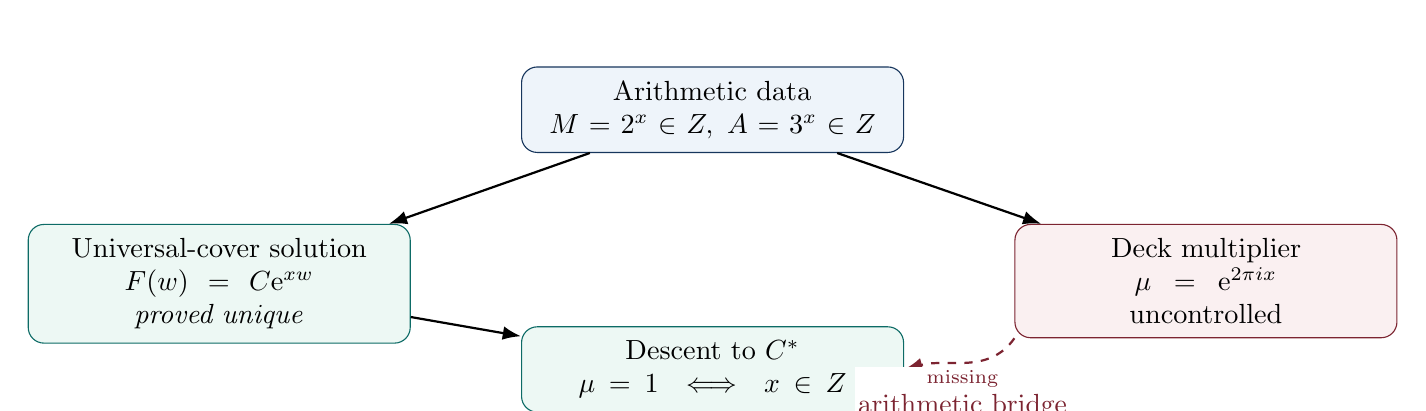
\begin{tikzpicture}[node distance=9mm and 14mm,>=Latex,
  box/.style={draw,rounded corners=2mm,align=center,inner sep=5pt,text width=4.5cm},
  good/.style={box,fill=softgreen,draw=teal},
  neutral/.style={box,fill=softblue,draw=navy},
  bad/.style={box,fill=softred,draw=burgundy}]
\node[neutral] (arith) {Arithmetic data\\ \(M=2^x\in\Z,\ A=3^x\in\Z\)};
\node[good,below left=of arith] (up) {Universal-cover solution\\ \(F(w)=C\e^{xw}\)\\ \emph{proved unique}};
\node[bad,below right=of arith] (mono) {Deck multiplier\\ \(\mu=\e^{2\pi ix}\)\\ uncontrolled};
\node[good,below=22mm of arith] (down) {Descent to \(\C^*\)\\ \(\mu=1\iff x\in\Z\)};
\draw[->,thick] (arith) -- (up);
\draw[->,thick] (arith) -- (mono);
\draw[->,thick] (up) -- (down);
\draw[->,thick,dashed,burgundy]
  (mono.south west) to[out=235,in=15]
  node[pos=.53,below=1pt,align=center,fill=white,inner sep=1pt,text=burgundy]
  {\scriptsize missing\\[-1pt] arithmetic bridge}
  (down.east);
\end{tikzpicture}%
}
\end{center}

\section{The arithmetic regularity ladder}

The same obstruction can be organized by asking in which local analytic category the germ \(z^x\) lies.  Each added regularity condition shrinks the allowed exponent spectrum.

\subsection{Laurent-spectrum rigidity}

\begin{theorem}[Meromorphic dilation eigenfunctions]
\label{thm:laurent}
Let \(q>1\), \(C\in\C^*\), and let \(f\) be a nonzero meromorphic germ at \(0\) satisfying
\[
  f(qz)=Cf(z).
\]
Then there are \(n\in\Z\) and \(c\in\C^*\) such that
\[
  f(z)=cz^n,\qquad C=q^n.
\]
If \(C\) is a positive integer and \(q\ge2\) is an integer, then \(n\ge0\).
\end{theorem}

\begin{proof}
Write the Laurent expansion
\(f(z)=\sum_{k=N}^{\infty}c_kz^k\).  Comparing coefficients in
\[
  \sum_{k=N}^{\infty}c_kq^kz^k
  =C\sum_{k=N}^{\infty}c_kz^k
\]
gives \((q^k-C)c_k=0\) for every \(k\).  Since \(k\mapsto q^k\) is injective, at most one coefficient is nonzero.  The final assertion follows because \(q^n<1\) for \(n<0\).
\end{proof}

The theorem shows that even one dilation would settle \eqref{eq:AE} if the power branch were meromorphic at the puncture.  The missing regularity is exactly what a nonintegral power lacks.

\subsection{Finite covers, Puiseux germs, and algebraicity}

\begin{proposition}[Finite ramification closes the problem]
\label{prop:finite-cover}
Suppose \(M=2^x\in\Z\).  If the germ \(z^x\) becomes single-valued after the finite cover \(z=w^q\) for some \(q\ge1\), then \(x\in\Nzero\).
\end{proposition}

\begin{proof}
After the cover, the germ is \(w^{qx}\).  Single-valuedness around \(w=0\) gives
\(\e^{2\pi i qx}=1\), so \(qx\in\Z\) and \(x\in\Q\).  Lemma~\ref{lem:basic} then gives \(x\in\Nzero\).
\end{proof}

\begin{corollary}[Algebraic power germs]
\label{cor:algebraic-germ}
For \(\lambda\in\C\), the germ \(z^\lambda\) is algebraic over \(\C(z)\) if and only if \(\lambda\in\Q\).  Consequently, a hypothetical nonintegral \AEconj{} solution gives a power germ transcendental over \(\C(z)\).
\end{corollary}

\begin{proof}
If \(\lambda=p/q\in\Q\), then \(y=z^\lambda\) satisfies an equation of the form
\(y^q=z^p\), after clearing a negative power if necessary.  Conversely, an algebraic germ has finite local monodromy.  Hence some positive power of the multiplier \(\e^{2\pi i\lambda}\) is \(1\), which forces \(\lambda\in\Q\).
\end{proof}

\subsection{Arithmetic D-finiteness}

The coefficient field matters.  The function \(z^x\) is always D-finite over \(\C(z)\), since it satisfies \(zy'-xy=0\).  The useful question is whether it is D-finite over the arithmetic field \(\Qbar(z)\).

\begin{theorem}[D-finite exponent criterion]
\label{thm:dfinite}
For \(\lambda\in\C\), the germ \(z^\lambda\) satisfies a nonzero linear differential equation over \(\Qbar(z)\) if and only if \(\lambda\in\Qbar\).
\end{theorem}

\begin{proof}
If \(\lambda\in\Qbar\), the first-order equation
\(zy'-\lambda y=0\) has coefficients in \(\Qbar(z)\).

Conversely, suppose
\[
  L=\sum_{j=0}^{r}p_j(z)\frac{\mathrm d^j}{\mathrm d z^j},
  \qquad p_j(z)\in\Qbar(z),\quad p_r\ne0,
\]
annihilates \(z^\lambda\).  Clear a common denominator so that every \(p_j\in\Qbar[z]\).  With
\(\fall{X}{j}=X(X-1)\cdots(X-j+1)\), define
\[
  Q(z,X):=\sum_{j=0}^{r}p_j(z)\fall{X}{j}z^{r-j}
  \in\Qbar[z,X].
\]
The coefficient of \(X^r\) in \(Q\) is \(p_r(z)\), so \(Q\) is not the zero polynomial.  Since
\[
  \frac{\mathrm d^j}{\mathrm d z^j}z^\lambda
  =\fall{\lambda}{j}z^{\lambda-j},
\]
we have
\[
  L(z^\lambda)=z^{\lambda-r}Q(z,\lambda).
\]
Thus \(Q(z,\lambda)=0\) identically in \(z\).  At least one coefficient of \(Q\), viewed as a polynomial in \(z\), is a nonzero polynomial in \(X\) with algebraic coefficients; that polynomial vanishes at \(\lambda\).  Hence \(\lambda\in\Qbar\).
\end{proof}

\begin{corollary}[Arithmetic holonomicity would prove \AEconj]
\label{cor:dfinite-close}
If \(M=2^x\in\Z\) and the germ \(z^x\) is D-finite over \(\Qbar(z)\), then \(x\in\Nzero\).
\end{corollary}

\begin{proof}
Theorem~\ref{thm:dfinite} makes \(x\) algebraic.  Gelfond--Schneider then excludes algebraic irrational \(x\), and Lemma~\ref{lem:basic} handles the rational case.
\end{proof}

\subsection{A nonlinear differential-equation trap}

\begin{proposition}[Nonlinear differential algebraicity is automatic]
\label{prop:nonlinear-ode}
Every power \(y=z^\lambda\), with arbitrary \(\lambda\in\C\), satisfies the nonlinear differential equation
\begin{equation}
  zyy''-z(y')^2+yy'=0,
  \label{eq:universal-nonlinear}
\end{equation}
whose coefficients lie in \(\Q[z]\).
\end{proposition}

\begin{proof}
For \(y=z^\lambda\),
\[
  zyy''=\lambda(\lambda-1)z^{2\lambda-1},\quad
  z(y')^2=\lambda^2z^{2\lambda-1},\quad
  yy'=\lambda z^{2\lambda-1}.
\]
The coefficients sum to \(\lambda(\lambda-1)-\lambda^2+\lambda=0\).
\end{proof}

\begin{auditbox}
A claim that ``\(z^x\) satisfies an algebraic differential equation over \(\Q(z)\), therefore \(x\) is algebraic'' is false.  Equation \eqref{eq:universal-nonlinear} works for every complex exponent.  Linearity and the arithmetic coefficient field in \cref{thm:dfinite} are both essential.
\end{auditbox}

\subsection{The spectrum ladder}

\begin{center}
\renewcommand{\arraystretch}{1.25}
\begin{tabularx}{0.98\textwidth}{>{\raggedright\arraybackslash}p{0.28\textwidth} >{\centering\arraybackslash}p{0.19\textwidth} X}
\toprule
\textbf{Category containing \(z^\lambda\)} & \textbf{Allowed \(\lambda\)} & \textbf{Consequence under \(2^x\in\Z\)}\\
\midrule
Meromorphic germ at \(0\) & \(\Z\) & Immediate integrality by Laurent comparison\\
Finite Puiseux cover / algebraic germ & \(\Q\) & Rational-exponent lemma gives \(x\in\Nzero\)\\
D-finite over \(\Qbar(z)\) & \(\Qbar\) & Gelfond--Schneider gives \(x\in\Nzero\)\\
Single-valued meromorphic on \(\C^*\) with both dilations & \(\Z\) & Complete classification, \cref{thm:downstairs}\\
Universal-cover holomorphic germ & \(\C\) & No exponent restriction; this is where a counterexample lives\\
Differentially algebraic over \(\Q(z)\) (nonlinear) & \(\C\) & No restriction; equation \eqref{eq:universal-nonlinear} is universal\\
\bottomrule
\end{tabularx}
\end{center}

This table locates the conjecture at a category boundary.  The arithmetic values make two exponentials of the Euler eigenvalue integral, but known arguments do not move the germ from the universal-cover category into any arithmetic regularity category above it.

\section{Arithmetic monodromy}

\subsection{The Six Exponentials consequence}

\begin{theorem}[Transcendental monodromy]
\label{thm:monodromy}
Assume \(x\) is a nonintegral solution of \eqref{eq:AE}.  Then for every nonzero rational \(r\),
\[
  \e^{2\pi i r x}
\]
is transcendental.  In particular, \(\mu=\e^{2\pi ix}\) is transcendental.
\end{theorem}

\begin{proof}
The numbers \(1,x\) are \(\Q\)-linearly independent.  The three numbers
\(\log2,\log3,2\pi ir\) are \(\Q\)-linearly independent: separating real and imaginary parts first kills the coefficient of \(2\pi ir\), and unique factorization kills the other two coefficients.  Apply the Six Exponentials Theorem to these two rows and three columns.  Five exponentials are algebraic:
\[
  2,\quad3,\quad \e^{2\pi ir},\quad M,\quad A.
\]
Therefore the sixth, \(\e^{2\pi irx}\), must be transcendental.
\end{proof}

\subsection{The algebraic multiplier plane}

\begin{theorem}[Exact algebraic directions in the three-translation space]
\label{thm:multiplier-plane}
Assume a nonintegral solution.  For \(r,s,t\in\Q\), set
\[
  \lambda=r\log2+s\log3+2\pi it.
\]
Then
\[
  \e^{x\lambda}\in\Qbar
  \quad\Longleftrightarrow\quad t=0.
\]
Thus, inside
\(\Span_{\Q}\{\log2,\log3,2\pi i\}\), the algebraic multipliers of the power character form exactly the real plane
\(\Span_{\Q}\{\log2,\log3\}\).
\end{theorem}

\begin{proof}
If \(t=0\), then
\[
  \e^{x\lambda}=M^rA^s\in\Qbar.
\]
If \(t\ne0\), factor
\[
  \e^{x\lambda}=M^rA^s\e^{2\pi itx}.
\]
The first factor is nonzero algebraic and the second is transcendental by \cref{thm:monodromy}; their product is transcendental.
\end{proof}

\subsection{One algebraic sheet and infinitely many arithmetic directions}

Let
\[
  \mathcal D_{2,3}:=\{2^r3^s:r,s\in\Q\}_{>0},
\]
the positive divisible hull of the \(3\)-smooth group.

\begin{theorem}[Dense, arithmetically independent branch orbit]
\label{thm:branch-orbit}
Assume a nonintegral solution and fix \(c\in\mathcal D_{2,3}\).  Analytic continuation of the principal value \(c^x\) around the origin produces
\[
  c^x\mu^k,\qquad k\in\Z.
\]
Then:
\begin{enumerate}[label=(\roman*)]
\item the orbit is dense on the circle \(|z|=c^x\);
\item the principal value \(c^x\) is algebraic;
\item every nonprincipal value \(c^x\mu^k\), \(k\ne0\), is transcendental;
\item the set \(\{c^x\mu^k:k\ge0\}\) is linearly independent over \(\Qbar\).
\end{enumerate}
\end{theorem}

\begin{proof}
Write \(c=2^r3^s\) with \(r,s\in\Q\).  Then \(c^x=M^rA^s\in\Qbar\).  Since \(x\notin\Q\), the powers of \(\mu=\e^{2\pi ix}\) are dense on the unit circle, proving (i).  For \(k\ne0\), \(\mu^k\) is transcendental by \cref{thm:monodromy}, so its product with the nonzero algebraic number \(c^x\) is transcendental.

For (iv), a finite \(\Qbar\)-linear relation would give
\(c^x P(\mu)=0\) for a nonzero polynomial \(P\in\Qbar[T]\).  This would make \(\mu\) algebraic, contradiction.
\end{proof}

\begin{auditbox}
The branch orbit is analytically one-dimensional over \(\C\) (every branch is a scalar multiple of the principal one), but arithmetically infinite-dimensional over \(\Qbar\).  No finite algebraic averaging of branches can cancel the monodromy.  Any successful ``take a trace over branches'' argument must first create finite or algebraic monodromy, which is already a decisive new input.
\end{auditbox}

\section{Integer sampling at the puncture}

\subsection{The accumulating lattice}

On the principal branch over the positive real axis, set
\[
  h(z):=z^{-x}.
\]
For \(a,b\in\Nzero\), define
\begin{equation}
  z_{a,b}:=2^{-a}3^{-b}.
  \label{eq:nodes-recip}
\end{equation}
Then \(z_{a,b}\to0\) along a two-dimensional logarithmic lattice, and
\begin{equation}
  h(z_{a,b})=M^aA^b\in\N.
  \label{eq:integer-puncture-values}
\end{equation}
Equivalently, the original branch has rational values
\[
  z_{a,b}^{x}=\frac1{M^aA^b}.
\]

\begin{proposition}[Node count and exact height slope]
\label{prop:node-count}
Let \(\alpha=\log2\), \(\beta=\log3\), and
\[
  N(T):=\#\{(a,b)\in\Nzero^2:a\alpha+b\beta\le T\}.
\]
Then
\begin{equation}
  N(T)=\frac{T^2}{2\alpha\beta}+O(T).
  \label{eq:node-count}
\end{equation}
Moreover,
\begin{equation}
  \log h(z_{a,b})
  =x\log\frac1{z_{a,b}}
  \label{eq:height-slope}
\end{equation}
holds exactly.
\end{proposition}

\begin{proof}
With \(A_T=\lfloor T/\alpha\rfloor\),
\[
N(T)=\sum_{a=0}^{A_T}
\left(\left\lfloor\frac{T-a\alpha}{\beta}\right\rfloor+1\right).
\]
Replacing each floor by its argument incurs \(O(A_T+1)=O(T)\), and the resulting arithmetic sum is
\[
 \frac1\beta\left((A_T+1)T-\frac{\alpha A_T(A_T+1)}2\right)+O(T)
 =\frac{T^2}{2\alpha\beta}+O(T).
\]
Finally,
\[
\log(M^aA^b)
=a\log M+b\log A
=x(a\log2+b\log3)
=x\log(1/z_{a,b}).
\]
\end{proof}

The arithmetic height grows at exactly the same exponent as the singularity.  There is no spare power in \eqref{eq:height-slope} for a naive denominator estimate to exploit.

\subsection{An explicit failure of uniqueness}

The sampling points accumulate at \(0\), but \(0\) is omitted from the natural domain of a nonintegral power.  The identity theorem therefore does not apply.  The following canonical product makes the failure quantitative and explicit.

Let
\begin{equation}
  \mathcal S:=\{2^a3^b:a,b\in\Nzero\}
  \label{eq:S}
\end{equation}
and define
\begin{equation}
  E(z):=\prod_{a,b\ge0}
  \left(1-\frac{z}{2^a3^b}\right).
  \label{eq:canonical-product}
\end{equation}
Because
\[
  \sum_{a,b\ge0}\frac1{2^a3^b}=3<\infty,
\]
the product converges uniformly on compact subsets of \(\C\) and defines an entire function with simple zero set \(\mathcal S\).

\begin{proposition}[Bounded integer samples at an essential singularity]
\label{prop:puncture-nonunique}
The function
\[
  P(z):=E(1/z)
\]
is holomorphic on \(\C^*\), has an essential singularity at \(0\), and vanishes at every node \(z_{a,b}=2^{-a}3^{-b}\).  Hence
\[
  G(z):=1+P(z)
\]
is a nonconstant holomorphic function on \(\C^*\), has an essential singularity at \(0\), and satisfies
\[
  G(z_{a,b})=1\in\Z
  \qquad(a,b\ge0).
\]
\end{proposition}

\begin{proof}
Composition with \(1/z\) makes \(P\) holomorphic on \(\C^*\).  Since \(E(2^a3^b)=0\), we get \(P(2^{-a}3^{-b})=0\).  If \(P\) were meromorphic at \(0\), then \(E(w)=P(1/w)\) would have at most polynomial growth at infinity and therefore be a polynomial.  But \(E\) has infinitely many zeros.  Thus the singularity is essential.  The assertions about \(G\) follow.
\end{proof}

\begin{auditbox}
Even bounded positive integer values on every point of the accumulating \(3\)-smooth reciprocal lattice do not force removability, meromorphicity, algebraicity, or finite ramification at the puncture.  Any proof based only on ``many integer values approaching zero'' is therefore invalid.  The exact dilation recurrences must be used.
\end{auditbox}

\section{The exact canonical-product growth threshold}

This section proves the main quantitative result of the report.

\subsection{A lattice integral}

For \(T\ge0\), define
\begin{equation}
  S(T):=\sum_{a,b\ge0}
  (T-a\alpha-b\beta)_+,
  \qquad u_+:=\max\{u,0\}.
  \label{eq:ST}
\end{equation}

\begin{lemma}[Integrated lattice count]
\label{lem:integrated-count}
As \(T\to\infty\),
\begin{equation}
  S(T)=\frac{T^3}{6\alpha\beta}+O(T^2).
  \label{eq:ST-asymp}
\end{equation}
\end{lemma}

\begin{proof}
For each pair \((a,b)\),
\[
  (T-a\alpha-b\beta)_+
  =\int_0^T\mathbf 1_{a\alpha+b\beta\le t}\,\dd t.
\]
Summing and using \cref{prop:node-count},
\[
  S(T)=\int_0^T N(t)\,\dd t
  =\int_0^T\left(\frac{t^2}{2\alpha\beta}+O(t+1)\right)\dd t
  =\frac{T^3}{6\alpha\beta}+O(T^2).
\]
\end{proof}

\subsection{Exact growth of the critical product}

For an entire function \(F\), write
\[
  M_F(R):=\max_{|z|=R}|F(z)|.
\]

\begin{theorem}[Critical canonical-product asymptotic]
\label{thm:E-growth}
The product \(E\) in \eqref{eq:canonical-product} satisfies
\begin{equation}
  \log M_E(R)
  =\frac{(\log R)^3}{6\log2\log3}
   +O((\log R)^2)
  \qquad(R\to\infty).
  \label{eq:E-growth}
\end{equation}
In fact, for every \(R>0\),
\[
  M_E(R)=E(-R)
  =\prod_{a,b\ge0}\left(1+\frac{R}{2^a3^b}\right).
\]
\end{theorem}

\begin{proof}
For \(|z|=R\), each factor obeys
\[
  \left|1-\frac{z}{2^a3^b}\right|
  \le 1+\frac{R}{2^a3^b}.
\]
At \(z=-R\), equality holds simultaneously for every factor.  Passing through the locally uniform product gives
\[
  M_E(R)=E(-R).
\]
Put \(R=\e^T\).  Then
\begin{equation}
  \log M_E(\e^T)
  =\sum_{a,b\ge0}
  \log\left(1+\e^{T-a\alpha-b\beta}\right).
  \label{eq:log-product-sum}
\end{equation}
For \(u=a\alpha+b\beta\le T\),
\[
  \log(1+\e^{T-u})=(T-u)+O(1).
\]
There are \(O(T^2)\) such pairs.  For \(u>T\), use
\(\log(1+\e^{T-u})\le\e^{T-u}\).  The tail is \(O(T+1)\): for each
\(a\le T/\alpha\), the geometric sum over
\(b>(T-a\alpha)/\beta\) is \(O(\e^{-(T-a\alpha)})\), which cancels the factor \(\e^{T-a\alpha}\); there are \(O(T)\) such \(a\).  The remaining \(a>T/\alpha\) form a convergent geometric tail.

Therefore \eqref{eq:log-product-sum} equals
\[
  \sum_{a,b\ge0}(T-a\alpha-b\beta)_+ +O(T^2).
\]
Apply \cref{lem:integrated-count} and replace \(T\) by \(\log R\).
\end{proof}

The ordinary order of \(E\) is zero.  The meaningful invariant is its \emph{cubic logarithmic type}.

\begin{definition}[Cubic logarithmic type]
\label{def:type}
For an entire function \(F\), define
\begin{equation}
  \tau_3(F):=
  \limsup_{R\to\infty}
  \frac{\log^+ M_F(R)}{(\log R)^3},
  \qquad \log^+u:=\max\{0,\log u\}.
  \label{eq:type}
\end{equation}
Set
\begin{equation}
  \tau_*:=\frac1{6\log2\log3}
  =0.2188662697\ldots.
  \label{eq:critical-type}
\end{equation}
\end{definition}

Theorem~\ref{thm:E-growth} says \(\tau_3(E)=\tau_*\).

\subsection{Jensen's lower bound}

\begin{theorem}[Sharp zero-set lower bound]
\label{thm:jensen-lower}
Let \(F\not\equiv0\) be entire and suppose
\[
  F(2^a3^b)=0\qquad(a,b\in\Nzero).
\]
Then
\begin{equation}
  \tau_3(F)\ge\tau_*.
  \label{eq:jensen-type}
\end{equation}
The constant is sharp, attained by \(E\).
\end{theorem}

\begin{proof}
Factor out a possible zero at the origin, which changes \(\log M_F(R)\) by only \(O(\log R)\).  We may assume \(F(0)\ne0\).  Jensen's formula implies
\[
  \log M_F(R)
  \ge \log|F(0)|+
  \sum_{2^a3^b<R}\log\frac{R}{2^a3^b}.
\]
With \(R=\e^T\), the sum is precisely \(S(T)\), up to points on the boundary, which contribute nothing.  Lemma~\ref{lem:integrated-count} gives
\[
  \log M_F(\e^T)
  \ge \frac{T^3}{6\alpha\beta}+O(T^2).
\]
Divide by \(T^3\) and take the limsup.  Sharpness follows from \cref{thm:E-growth}.
\end{proof}

\begin{resultbox}
The reciprocal \(3\)-smooth lattice is neither a uniqueness set for arbitrary holomorphic functions nor a zero set of negligible growth.  It has an exact critical scale: a nonzero entire function can vanish there with ordinary order zero, but it must pay at least the cubic logarithmic type
\(\tau_*=1/(6\log2\log3)\).  The canonical product pays exactly that amount.
\end{resultbox}

\section{A sharp entire-interpolation criterion for \AEconj}

\subsection{The interpolation data}

The hypothetical arithmetic data can be written on \(\mathcal S\) as
\begin{equation}
  y(2^a3^b):=M^aA^b=(2^a3^b)^x.
  \label{eq:data-S}
\end{equation}
Since \(\mathcal S\) is discrete in \(\C\), the classical entire interpolation theorem guarantees the existence of some entire \(H\) taking these prescribed values.  Existence without a growth bound is easy; the growth is the entire issue.

\begin{theorem}[Subcritical interpolation rigidity]
\label{thm:subcritical}
Let \(p,q>1\) be multiplicatively independent positive real numbers, let \(P,Q\in\C^*\), and suppose an entire function \(H\) satisfies
\begin{equation}
  H(p^aq^b)=P^aQ^b
  \qquad(a,b\in\Nzero).
  \label{eq:general-interp}
\end{equation}
Define
\[
  \tau_{p,q}:=\frac1{6\log p\log q}.
\]
If
\begin{equation}
  \limsup_{R\to\infty}
  \frac{\log^+M_H(R)}{(\log R)^3}
  <\tau_{p,q},
  \label{eq:subcritical-bound}
\end{equation}
then there is an \(n\in\Nzero\) such that
\[
  H(z)=z^n,
  \qquad P=p^n,
  \qquad Q=q^n.
\]
\end{theorem}

\begin{proof}
Consider the first dilation defect
\begin{equation}
  D_p(z):=H(pz)-P H(z).
  \label{eq:Dp}
\end{equation}
For every \(a,b\ge0\), the interpolation rule gives
\[
  D_p(p^aq^b)
  =P^{a+1}Q^b-P\,P^aQ^b=0.
\]
The maximum modulus satisfies
\[
  M_{D_p}(R)
  \le M_H(pR)+|P|M_H(R).
\]
Replacing \(R\) by \(pR\) does not change the leading coefficient on the \((\log R)^3\) scale.  Therefore \(D_p\) has cubic logarithmic type at most that of \(H\), strictly below \(\tau_{p,q}\).

The proof of \cref{thm:jensen-lower}, with \(\log2,\log3\) replaced by \(\log p,\log q\), shows that a nonzero entire function vanishing on every \(p^aq^b\) must have type at least \(\tau_{p,q}\).  Hence \(D_p\equiv0\):
\[
  H(pz)=PH(z).
\]
Expand \(H(z)=\sum_{n\ge0}c_nz^n\).  Coefficient comparison gives
\[
  (p^n-P)c_n=0
  \quad(n\ge0).
\]
Since \(H(1)=1\), the function is nonzero.  Thus \(P=p^n\) for a unique \(n\in\Nzero\), and \(H(z)=cz^n\).  The value at \(1=p^0q^0\) gives \(c=1\).  Finally, the value at \(q\) gives \(Q=H(q)=q^n\).
\end{proof}

\begin{corollary}[Sharp analytic criterion for the conjecture]
\label{cor:AE-interp}
Assume \(M=2^x\in\Z\) and \(A=3^x\in\Z\).  If there exists an entire function \(H\) such that
\[
  H(2^a3^b)=M^aA^b
  \quad(a,b\ge0)
\]
and
\[
  \tau_3(H)<\frac1{6\log2\log3},
\]
then \(x\in\Nzero\) and \(H(z)=z^x\).
Conversely, when \(x\in\Nzero\), the polynomial \(H(z)=z^x\) has type \(0\) and supplies such an interpolant.
\end{corollary}

\begin{proof}
Apply \cref{thm:subcritical} with \(p=2,q=3,P=M,Q=A\).  It gives \(M=2^n\) and \(A=3^n\), so injectivity of \(t\mapsto2^t\) on \(\R\) gives \(x=n\).
\end{proof}

\subsection{Sharpness for integrality alone}

\begin{proposition}[The threshold cannot be weakened generically]
\label{prop:sharpness}
The function
\[
  J(z):=1+E(z)
\]
is a transcendental entire function satisfying
\[
  J(2^a3^b)=1\in\Z
  \quad(a,b\ge0),
\]
and
\[
  \tau_3(J)=\tau_*.
\]
Thus a P\'olya-type theorem based only on integer values on \(\mathcal S\) cannot replace the strict inequality \(\tau_3<\tau_*\) by any larger universal threshold.
\end{proposition}

\begin{proof}
The values follow from the zero set of \(E\).  Since \(E\) is nonpolynomial, \(J\) is transcendental entire.  Addition of a constant does not change the leading cubic logarithmic type.
\end{proof}

This matches the philosophy of P\'olya's theorem on \(\Nzero\) and Gel'fond-type theorems on a geometric progression: the smallest transcendental integer-valued entire function sets the exact growth barrier.  Pila's work develops this philosophy for concordant value sequences and geometric progressions \cite{Pila2003}.  Here the two-generator semigroup creates a cubic logarithmic, rather than ordinary exponential, threshold.

\subsection{A growth dichotomy}

\begin{corollary}[Polynomial-versus-critical-growth dichotomy]
\label{cor:growth-dichotomy}
Under the hypotheses of \eqref{eq:AE}, exactly one of the following global alternatives holds:
\begin{enumerate}[label=(\roman*)]
\item \(x\in\Nzero\), in which case the polynomial \(z^x\) is an interpolant of type \(0\);
\item \(x\notin\Z\), in which case every entire interpolant \(H\) of \eqref{eq:data-S} satisfies
\[
  \tau_3(H)\ge\tau_*.
\]
\end{enumerate}
\end{corollary}

\begin{proof}
The alternatives are mutually exclusive.  The first assertion is immediate.  If \(x\notin\Z\) and some interpolant had type below \(\tau_*\), \cref{cor:AE-interp} would force \(x\in\Z\), contradiction.
\end{proof}

\begin{gapbox}
The new criterion reduces the conjecture to a concrete analytic construction: use the arithmetic of the values \(M^aA^b\) to produce an entire interpolant of cubic logarithmic type \emph{strictly below} \(\tau_*\).  General interpolation theorems do not supply that saving.  The canonical product shows that a critical-type obstruction is real, not an artifact of a loose estimate.
\end{gapbox}

\section{At the critical boundary: an exact defect cocycle}
\label{sec:critical-cocycle}

The strict inequality in \cref{thm:subcritical} kills each dilation defect by Jensen's theorem.  At the critical type, the defect need not vanish, but its compulsory canonical-product factor can be removed exactly.  What remains is a lower-dimensional boundary problem.

\subsection{One-dimensional edge products}

Define
\begin{equation}
  B_2(z):=\prod_{b\ge0}\left(1-\frac{2z}{3^b}\right),
  \qquad
  B_3(z):=\prod_{a\ge0}\left(1-\frac{3z}{2^a}\right).
  \label{eq:edge-products}
\end{equation}
Both products converge locally uniformly.  Splitting off the boundary row or column of the two-dimensional product gives the exact identities
\begin{equation}
  E(2z)=E(z)B_2(z),
  \qquad
  E(3z)=E(z)B_3(z).
  \label{eq:E-dilation-edge}
\end{equation}
Thus dilation of the critical product preserves the full interior zero lattice and creates only a one-dimensional edge divisor.

\begin{proposition}[Quadratic logarithmic growth of the edges]
\label{prop:edge-growth}
As \(R\to\infty\),
\begin{align}
  \log M_{B_2}(R)
    &=\frac{(\log R)^2}{2\log3}+O(\log R),
    \label{eq:B2-growth}\\
  \log M_{B_3}(R)
    &=\frac{(\log R)^2}{2\log2}+O(\log R).
    \label{eq:B3-growth}
\end{align}
Moreover, \(M_{B_j}(R)=B_j(-R)\) for \(j=2,3\).
\end{proposition}

\begin{proof}
The factorwise triangle inequality is again sharp at \(-R\).  For example,
\[
  \log B_2(-R)
   =\sum_{b\ge0}\log\left(1+\exp(\log R+\log2-b\log3)\right).
\]
Writing \(T=\log R+\log2\), the terms with \(b\log3\le T\) contribute
\[
  \sum_{0\le b\le T/\log3}(T-b\log3)+O(T)
  =\frac{T^2}{2\log3}+O(T).
\]
The geometric tail is \(O(1)\).  Since replacing \(T\) by \(\log R+O(1)\) affects only the \(O(\log R)\) term, \eqref{eq:B2-growth} follows.  The proof of \eqref{eq:B3-growth} is identical.
\end{proof}

The inequality \(\log2<\log3\) makes the \(B_3\)-edge asymptotically larger:
\begin{equation}
  \frac1{2\log2}>\frac1{2\log3}.
  \label{eq:edge-gap}
\end{equation}
This strict second-order gap will separate finite-dimensional defect quotients.

\subsection{Factorization and the commuting cocycle}

Let \(H\) be any entire interpolant of the multiplicative data,
\[
  H(2^a3^b)=M^aA^b.
\]
Set
\begin{equation}
  D_2(z):=H(2z)-MH(z),
  \qquad
  D_3(z):=H(3z)-AH(z).
  \label{eq:two-defects}
\end{equation}
Both defects vanish at every zero of \(E\).

\begin{theorem}[Exact critical defect cocycle]
\label{thm:defect-cocycle}
There are unique entire functions \(U,V\) such that
\begin{equation}
  D_2=EU,
  \qquad
  D_3=EV.
  \label{eq:defect-factorization}
\end{equation}
They satisfy the exact compatibility equation
\begin{equation}
  B_3(z)U(3z)-A U(z)
  =B_2(z)V(2z)-M V(z).
  \label{eq:defect-cocycle}
\end{equation}
Conversely, \eqref{eq:defect-cocycle} is precisely the compatibility forced by commutativity of the two dilations.
\end{theorem}

\begin{proof}
Every zero \(2^a3^b\) of \(E\) is simple, while \(D_2\) and \(D_3\) vanish there.  Hence the quotients \(D_2/E\) and \(D_3/E\) have removable singularities at all zeros of \(E\), giving unique entire functions \(U,V\).

The two defects obey the tautological commuting-square identity
\begin{align*}
  D_2(3z)-A D_2(z)
  &=H(6z)-M H(3z)-A H(2z)+AMH(z)\\
  &=D_3(2z)-M D_3(z).
\end{align*}
Substitute \eqref{eq:defect-factorization}, use \eqref{eq:E-dilation-edge}, and divide by \(E(z)\).  The resulting identity is \eqref{eq:defect-cocycle}.
\end{proof}

Equation \eqref{eq:defect-cocycle} is an infinite analogue of a boundary-residual identity: the two-dimensional interior divisor has been cancelled, and only the two one-dimensional edge products remain.  This is strictly more informative than saying merely that each defect vanishes on the sampling set.

\subsection{A finite-dimensional critical-type closure theorem}

\begin{theorem}[Polynomial boundary quotients force a monomial]
\label{thm:polynomial-quotients}
In the setting of \cref{thm:defect-cocycle}, suppose that the entire quotients \(U\) and \(V\) are polynomials.  Then
\[
  U=V=0.
\]
Consequently, there is an \(n\in\Nzero\) such that
\[
  H(z)=z^n,\qquad M=2^n,\qquad A=3^n.
\]
In particular, for the \AEconj{} data this condition proves \(x=n\in\Nzero\), even though \(H\) itself is allowed to have the critical cubic logarithmic type.
\end{theorem}

\begin{proof}
Assume first that \(U\ne0\), and let \(d=\deg U\).  Put \(z=-R\) in \eqref{eq:defect-cocycle} and rearrange:
\begin{equation}
  B_3(-R)U(-3R)
  =A U(-R)+B_2(-R)V(-2R)-M V(-R).
  \label{eq:negative-axis-cocycle}
\end{equation}
For large \(R\), the left side has modulus at least
\[
  cR^d\exp\left(\frac{(\log R)^2}{2\log2}+O(\log R)\right)
\]
for some \(c>0\).  The right side is bounded by a polynomial in \(R\) times
\[
  \exp\left(\frac{(\log R)^2}{2\log3}+O(\log R)\right).
\]
The strict gap \eqref{eq:edge-gap} makes this impossible as \(R\to\infty\).  Therefore \(U=0\).

Equation \eqref{eq:defect-cocycle} now reduces to
\[
  B_2(z)V(2z)=M V(z).
\]
If \(V\ne0\), evaluation at \(-R\) makes the left side grow like a nonzero polynomial times
\(\exp((\log R)^2/(2\log3)+O(\log R))\), whereas the right side has only polynomial growth.  Hence \(V=0\).

Thus both dilation defects vanish.  From \(H(2z)=MH(z)\) and the Taylor expansion of \(H\), coefficient comparison gives \(H(z)=cz^n\) and \(M=2^n\) for some \(n\in\Nzero\).  Since \(H(1)=1\), \(c=1\), and \(H(3)=A\) yields \(A=3^n\).
\end{proof}

\begin{resultbox}
There are now two quantitatively different ways to close the interpolation route.  A cubic-type saving below \(\tau_*\) annihilates the defects before division by \(E\).  At the exact critical type, it is enough to show that the divided defects \(U=D_2/E\) and \(V=D_3/E\) lie in a finite-dimensional polynomial class.  The strict quadratic edge-growth gap then annihilates them.
\end{resultbox}

\subsection{Why critical type alone still does not close the problem}

Even for an integral exponent \(n\), critical-type interpolants need not have zero defects.  For any \(c\in\C^*\),
\begin{equation}
  H_c(z):=z^n+cE(z)
  \label{eq:critical-family}
\end{equation}
interpolates the same data \(H_c(2^a3^b)=(2^a3^b)^n\) and has \(\tau_3(H_c)=\tau_*\).  Its quotient defects are
\begin{equation}
  U_c(z)=c\bigl(B_2(z)-2^n\bigr),
  \qquad
  V_c(z)=c\bigl(B_3(z)-3^n\bigr),
  \label{eq:critical-family-quotients}
\end{equation}
which are transcendental entire functions of quadratic logarithmic growth.  Thus a bare bound \(\tau_3(H)\le\tau_*\) cannot distinguish the polynomial interpolant from a critical perturbation.  The divided-defect regularity in \cref{thm:polynomial-quotients} is a genuine second-order condition, not a cosmetic strengthening.


\section{Why the obvious closures fail}

\subsection{Identity theorem}

The nodes \(2^{-a}3^{-b}\) accumulate only at the deleted point \(0\).  Proposition~\ref{prop:puncture-nonunique} gives a nonzero holomorphic function on \(\C^*\) vanishing on all of them.  Therefore neither values nor zeros on that lattice determine a punctured-domain holomorphic function.

\subsection{``Two q-difference equations imply rationality''}

The power branch satisfies
\[
  f(2z)=Mf(z),\qquad f(3z)=Af(z)
\]
with algebraic coefficients.  Rationality theorems for simultaneous Mahler or \(q\)-difference equations impose a formal-power-series, single-valued meromorphic, or comparable regularity category.  For example, the simultaneous Mahler theorem concerns \(f(z^p)\) and \(f(z^q)\) for a formal power series, while consistent \(q\)-difference systems are analyzed in single-valued meromorphic settings \cite{SchaefkeSinger2019,SchaefkeSingerMahler2017,Jolly2002}.  A nonintegral \(z^x\) lives only on the universal cover and is exactly excluded by those hypotheses.

\begin{warning}
The substitutions \(z\mapsto2z,3z\) are multiplicative dilations, not the Mahler substitutions \(z\mapsto z^2,z^3\).  More importantly, even the correct \(q\)-difference theorem cannot be applied before proving that the solution descends to its required single-valued category.
\end{warning}

\subsection{Weak growth at the puncture}

The function \(P(z)=E(1/z)\) has an essential singularity but corresponds to an entire function \(E\) of ordinary order zero.  Thus ``finite order'' or any ordinary-order bound in \(1/z\) is too weak.  The relevant threshold is the sharper cubic logarithmic type computed in \cref{thm:E-growth}.

\subsection{Nonlinear differential algebraicity}

Proposition~\ref{prop:nonlinear-ode} gives a universal rational nonlinear ODE for all powers.  Only an arithmetic \emph{linear} differential equation would close the problem.

\subsection{A third algebraic multiplier}

If one could manufacture any translation direction in
\(\Span_\Q\{\log2,\log3,2\pi i\}\) with a nonzero \(2\pi i\)-component and an algebraic multiplier, \cref{thm:multiplier-plane} would give an immediate contradiction.  But no such direction follows from the two integer values.  This is another exact form of the Four Exponentials wall.

\section{A concrete research program}

The preceding theorems produce four closure targets, ranging from global growth control to local arithmetic descent.

\subsection{Target I: subcritical entire interpolation}

\begin{problem}[Subcritical interpolation problem]
\label{prob:subcritical}
Assume \(M=2^x\), \(A=3^x\) are integers.  Construct, using only this arithmetic hypothesis, an entire \(H\) with
\[
  H(2^a3^b)=M^aA^b
\]
and
\[
  \tau_3(H)<\frac1{6\log2\log3}.
\]
\end{problem}

By \cref{cor:AE-interp}, solving this problem proves \AEconj.  A viable construction must beat the critical canonical product by a strict amount.  Merely producing an order-zero interpolant is not enough.

A plausible technical direction is an arithmetic Newton or Lagrange interpolation in which divisibility of the integer data yields cancellation in the coefficients.  Classical integer-valued entire-function theory shows that such cancellations can create sharp growth gaps on \(\Nzero\) and on one geometric progression \cite{Polya1915,PilaRodriguez1999,Pila2003}.  The new difficulty is the irregular one-dimensional ordering of the two-dimensional semigroup \(2^a3^b\).

\subsection{Target I-b: finite-dimensional divided defects}

\begin{problem}[Critical-boundary quotient problem]
\label{prob:quotients}
Construct an entire interpolant \(H\) for which the quotients
\[
  \frac{H(2z)-MH(z)}{E(z)},\qquad
  \frac{H(3z)-AH(z)}{E(z)}
\]
are polynomials, or belong to another explicitly controlled finite-dimensional class for which the edge cocycle \eqref{eq:defect-cocycle} has only the zero solution.
\end{problem}

By \cref{thm:polynomial-quotients}, polynomial quotients already prove the conjecture without any strict cubic-type saving.  This target is potentially more flexible than \cref{prob:subcritical}: the interpolant may lie at the unavoidable critical type, provided that all of its nontrivial defect is confined to finitely many boundary modes.  Formula \eqref{eq:critical-family-quotients} shows why a generic critical perturbation fails this requirement---its quotients carry the full one-dimensional edge products.

\subsection{Target II: arithmetic holonomicity}

\begin{problem}[Arithmetic linear ODE]
\label{prob:ODE}
Derive from \(M,A\in\Z\) a nonzero operator
\[
  L\in\Qbar(z)\left[\frac{\mathrm d}{\mathrm d z}\right]
\]
that annihilates the branch \(z^x\).
\end{problem}

Theorem~\ref{thm:dfinite} and Gelfond--Schneider would then prove \(x\in\Nzero\).  The operator must be linear; nonlinear differential algebraicity carries no information.

An equivalent Euler-operator version is useful.  Let \(\Theta=z\frac{\mathrm d}{\mathrm d z}\).  The branch satisfies \(\Theta f=xf\), while the dilation operators satisfy formally
\[
  f(qz)=q^\Theta f.
\]
The arithmetic hypothesis says that \(2^\Theta\) and \(3^\Theta\) have integer eigenvalues on \(f\).  To recover an algebraic eigenvalue of \(\Theta\), one needs a finite-dimensional arithmetic functional calculus; the universal-cover function space has point spectrum all of \(\C\), so no such conclusion is automatic.

\subsection{Target III: algebraic monodromy}

\begin{problem}[Monodromy algebraicity]
\label{prob:monodromy}
Prove from \(M,A\in\Z\) that
\[
  \mu=\e^{2\pi ix}
\]
is algebraic.
\end{problem}

Under a nonintegral solution, \cref{thm:monodromy} says \(\mu\) is transcendental.  Thus algebraicity alone, not necessarily triviality, would already close the conjecture.  Finite ramification, algebraic-function descent, or an arithmetic trace construction would each imply such algebraicity, but none is presently derived from the samples.

\subsection{Why these targets are genuinely different}

Subcritical interpolation controls a global single-valued entire surrogate on the \(z\)-plane.  The critical-boundary target controls the residual edge modes after the compulsory divisor \(E\) is removed.  Arithmetic holonomicity controls the local differential category of the actual branch.  Monodromy algebraicity controls only the deck transformation.  Any one would suffice, but the proofs required are not interchangeable:
\begin{itemize}
\item an entire interpolant need not equal \(z^x\) until its dilation defects are killed;
\item critical cubic type can still be useful if the divided defects have finite-dimensional boundary complexity;
\item a nonlinear ODE does not control the exponent;
\item monodromy information is invisible to the real dilation equations upstairs.
\end{itemize}

\section{Relation to current literature}

\subsection{Four Exponentials and the matrix-coefficient program}

Waldschmidt formulates the exact integer-power question and places it under the Four Exponentials problem \cite{Waldschmidt2023}.  Dasgupta and Kakde's Matrix Coefficient Conjecture states that a singular matrix of logarithms of algebraic numbers has a zero rational matrix coefficient after rational changes of basis; in dimension two it is equivalent to Four Exponentials.  Their work proves several structural implications and develops a fewnomial auxiliary-polynomial strategy, but leaves the decisive implication open \cite{DasguptaKakde2026}.  The local-descent route in this report does not resolve that missing implication; rather, it gives a different analytic avatar of the same rank-two obstruction.

\subsection{Recent transcendence-degree work}

Massold proves a weaker lower bound for transcendence degrees of fields generated by exponentials of products and reduces a stronger bound to a conjecture on intersections in split tori \cite{Massold2025}.  This is relevant context but does not supply the rank-two conclusion needed here.

\subsection{Difference equations and regularity hypotheses}

Sch\"afke and Singer prove rationality and structure results for consistent systems of differential, \(q\)-difference, and Mahler equations under precise formal or meromorphic hypotheses \cite{SchaefkeSinger2019,SchaefkeSingerMahler2017}.  Jolly studies meromorphic solutions of two-step constant-coefficient difference systems \cite{Jolly2002}.  These theories support the central lesson of \cref{thm:downstairs}: simultaneous recurrences become powerful only after a single-valued meromorphic category has been established.

\subsection{Integer-valued entire functions}

P\'olya initiated sharp growth theorems for entire functions taking integer values on \(\Nzero\) \cite{Polya1915}.  Pila and Rodriguez Villegas, and later Pila, developed concordance and sharp ``smallest transcendental function'' principles for sparse sets including geometric progressions \cite{PilaRodriguez1999,Pila2003}.  The canonical product calculation in this report is a two-generator semigroup analogue: the critical scale is
\((\log R)^3\), with type \(1/(6\log2\log3)\).

\subsection{A recent automaticity result that does not settle the problem}

Bustos-Gajardo, Fokkink, and Yassawi proved a 2026 Cobham theorem for Gaussian integer numeration systems without relying on Four Exponentials in the cases they need \cite{BustosFokkinkYassawi2026}.  This is a genuine advance in automaticity, but it bypasses rather than proves Four Exponentials and therefore does not settle \eqref{eq:AE}.

\section{Claim ledger and final assessment}

\subsection{Unconditional results proved here}

\begin{longtable}{>{\raggedright\arraybackslash}p{0.34\textwidth} >{\raggedright\arraybackslash}p{0.56\textwidth}}
\toprule
\textbf{Result} & \textbf{Content}\\
\midrule
\endhead
Universal-cover rigidity & Every nonzero entire solution of the two incommensurable translation equations is a single exponential; \cref{thm:upstairs}.\\
Downstairs classification & Every single-valued meromorphic solution on \(\C^*\) is a monomial; integer multipliers force a nonnegative integer exponent; \cref{thm:downstairs}.\\
Arithmetic regularity ladder & Meromorphic, finite-Puiseux, algebraic, and \(\Qbar\)-D-finite descent each force rational or algebraic exponents and hence close \AEconj; \cref{thm:laurent,prop:finite-cover,thm:dfinite}.\\
Nonlinear-ODE audit & Every power satisfies the same nonlinear rational ODE, so nonlinear differential algebraicity is useless; \cref{prop:nonlinear-ode}.\\
Arithmetic branch orbit & Under a counterexample, monodromy is transcendental and its branch values are dense and \(\Qbar\)-linearly independent; \cref{thm:monodromy,thm:branch-orbit}.\\
Explicit nonuniqueness & A holomorphic function with an essential puncture can take the bounded integer value \(1\) on every reciprocal \(3\)-smooth node; \cref{prop:puncture-nonunique}.\\
Critical product growth & The canonical product has exact growth constant \(1/(6\log2\log3)\); \cref{thm:E-growth}.\\
Sharp Jensen lower bound & Every nonzero entire function vanishing on all \(3\)-smooth integers pays at least the critical cubic logarithmic type; \cref{thm:jensen-lower}.\\
Subcritical interpolation theorem & An entire interpolant of the multiplicative data below the critical type must be a monomial, forcing \(x\in\Nzero\); \cref{thm:subcritical,cor:AE-interp}.\\
Critical defect cocycle & For every entire interpolant, each defect factors by \(E\), and the quotients satisfy an exact edge-product compatibility equation; \cref{thm:defect-cocycle}.\\
Polynomial-quotient closure & Polynomial divided defects must vanish because the two edge products have unequal quadratic logarithmic growth; \cref{thm:polynomial-quotients}.\\
Sharpness & The critical constant is attained by a transcendental entire function integer-valued on the whole semigroup; \cref{prop:sharpness}.\\
\bottomrule
\end{longtable}

\subsection{What is not proved}

No argument in this report derives one of the following from the bare hypothesis \(M,A\in\Z\):
\begin{enumerate}
\item a subcritical entire interpolant;
\item a critical interpolant whose divided defects are polynomial or otherwise finite-dimensional;
\item a linear differential equation over \(\Qbar(z)\) for \(z^x\);
\item algebraic or finite monodromy;
\item single-valued meromorphic descent to \(\C^*\).
\end{enumerate}
Each item would prove the conjecture.  Establishing any one without importing the conclusion remains the unresolved step.

\begin{verdictbox}
The requested implication has not been proved unconditionally, because doing so would solve a recognized open special case of Four Exponentials.  The work above nevertheless produces a distinct, exact analytic reduction with a sharp numerical threshold:
\[
\boxed{\displaystyle
\tau_* = \frac1{6\log2\log3}.}
\]
A hypothetical counterexample forces every entire interpolation of its multiplicative integer data to live at or above this critical cubic logarithmic type.  Any arithmetic construction that saves a positive amount below \(\tau_*\) proves \(x\in\Z\).  At exact critical type, polynomial divided defects also suffice, by the quadratic edge-growth gap.  The canonical product and the family \(z^n+cE\) show why a bare non-strict or ordinary-order argument cannot succeed.
\end{verdictbox}

\appendix

\section{General \texorpdfstring{\(d\)}{d}-generator form of the growth calculation}

The two-generator constant is part of a clean general pattern.

Let \(q_1,\dots,q_d>1\) be multiplicatively independent and put
\[
  \mathcal S_d=\{q_1^{a_1}\cdots q_d^{a_d}:a_j\in\Nzero\}.
\]
Then
\[
  N_d(T):=\#\left\{a\in\Nzero^d:
  \sum_{j=1}^d a_j\log q_j\le T\right\}
  =\frac{T^d}{d!\prod_{j=1}^d\log q_j}+O(T^{d-1}).
\]
Integrating gives
\[
  \sum_{a\in\Nzero^d}
  \left(T-\sum_j a_j\log q_j\right)_+
  =\frac{T^{d+1}}{(d+1)!\prod_j\log q_j}+O(T^d).
\]
Thus the canonical product over \(\mathcal S_d\) has logarithmic degree \(d+1\) and critical type
\[
  \frac1{(d+1)!\prod_j\log q_j}.
\]
The proof of \cref{thm:subcritical} generalizes verbatim: a subcritical entire interpolant of multiplicative eigen-data on a \(d\)-generator semigroup must be a monomial.  The \AEconj{} case is \(d=2\).

\section{A reusable proof-audit checklist}

Any proposed proof of \eqref{eq:AE} using analytic functions should answer the following questions explicitly.

\begin{enumerate}[label=\textbf{A\arabic*.}]
\item On what domain is \(z^x\) being treated as single-valued?  If the domain winds around \(0\), where was trivial monodromy proved?
\item Is the functional equation a dilation \(f(qz)\) or a Mahler equation \(f(z^q)\)?
\item Does the invoked difference-equation theorem require a formal power series, a meromorphic function on \(\C^*\), or finite order?
\item If an identity theorem is used, is the accumulation point inside the domain?
\item If a differential equation is used, is it linear and defined over an arithmetic coefficient field?
\item If zeros on \(\{2^a3^b\}\) are used, is the growth estimate strictly below the critical cubic logarithmic type \(\tau_*\)?
\item If branches are averaged, why is the monodromy algebraic or finite?  Under a counterexample, its powers are \(\Qbar\)-linearly independent.
\item If an auxiliary entire interpolant is constructed, what quantitative bound is proved for its dilation defects?
\end{enumerate}

\section{Bibliographic notes}

\begin{thebibliography}{99}

\bibitem{AlaogluErdos1944}
L.~Alaoglu and P.~Erd\H{o}s,
\newblock On highly composite and similar numbers,
\newblock \emph{Transactions of the American Mathematical Society} \textbf{56} (1944), 448--469.

\bibitem{BustosFokkinkYassawi2026}
\'A.~Bustos-Gajardo, R.~Fokkink, and R.~Yassawi,
\newblock Cobham's theorem for the Gaussian integers,
\newblock arXiv:2510.01440v3, 2026.

\bibitem{DasguptaKakde2026}
S.~Dasgupta and M.~Kakde,
\newblock Ranks of matrices of logarithms of algebraic numbers II: the Matrix Coefficient Conjecture,
\newblock \emph{Advances in Mathematics} \textbf{487} (2026), Article 110753,
DOI 10.1016/j.aim.2025.110753.

\bibitem{Gelfond1934}
A.~O.~Gel'fond,
\newblock Sur le septi\`eme probl\`eme de Hilbert,
\newblock \emph{Izvestiya Akademii Nauk SSSR} \textbf{7} (1934), 623--630.

\bibitem{Jolly2002}
J.-C.~Jolly,
\newblock Solutions m\'eromorphes sur \(\C\) d'un syst\`eme d'\'equations aux diff\'erences \`a coefficients constants et \`a deux pas r\'ecurrents,
\newblock \emph{Annales de l'Institut Fourier} \textbf{52} (2002), no.~2, 585--622,
DOI 10.5802/aif.1895.

\bibitem{Massold2025}
H.~Massold,
\newblock Transcendence degrees of fields generated by exponentials of products,
\newblock arXiv:2506.01123, 2025.

\bibitem{PilaRodriguez1999}
J.~Pila and F.~Rodriguez Villegas,
\newblock Concordant sequences and integral-valued entire functions,
\newblock \emph{Acta Arithmetica} \textbf{88} (1999), 239--268.

\bibitem{Pila2003}
J.~Pila,
\newblock Entire functions having a concordant value sequence,
\newblock \emph{Israel Journal of Mathematics} \textbf{134} (2003), 317--343.

\bibitem{Polya1915}
G.~P\'olya,
\newblock Ueber ganzwertige ganze Funktionen,
\newblock \emph{Rendiconti del Circolo Matematico di Palermo} \textbf{40} (1915), 1--16.

\bibitem{SchaefkeSingerMahler2017}
R.~Sch\"afke and M.~F.~Singer,
\newblock Mahler equations and rationality,
\newblock arXiv:1605.08830v2, 2017.

\bibitem{SchaefkeSinger2019}
R.~Sch\"afke and M.~F.~Singer,
\newblock Consistent systems of linear differential and difference equations,
\newblock \emph{Journal of the European Mathematical Society} \textbf{21} (2019), 2751--2792.

\bibitem{Schneider1934}
T.~Schneider,
\newblock Transzendenzuntersuchungen periodischer Funktionen. I, II,
\newblock \emph{Journal f\"ur die reine und angewandte Mathematik} \textbf{172} (1934), 65--69, 70--74.

\bibitem{Waldschmidt2000}
M.~Waldschmidt,
\newblock \emph{Diophantine Approximation on Linear Algebraic Groups},
\newblock Grundlehren der mathematischen Wissenschaften 326, Springer, 2000.

\bibitem{Waldschmidt2005}
M.~Waldschmidt,
\newblock Variations on the Six Exponentials Theorem,
\newblock in \emph{Algebra and Number Theory}, Hindustan Book Agency, 2005, 338--355.

\bibitem{Waldschmidt2023}
M.~Waldschmidt,
\newblock The Four Exponentials Problem and Schanuel's Conjecture,
\newblock in \emph{Mathematics Going Forward}, Lecture Notes in Mathematics 2313, Springer, 2023, 579--592,
DOI 10.1007/978-3-031-12244-6\_39.

\end{thebibliography}

\end{document}
